\documentclass{beamer}

\usepackage{amsmath}

\usetheme{AnnArbor}
\usecolortheme{crane}
\usefonttheme[onlymath]{serif}

\title{Deep Learning - Foundations and Concepts}
\subtitle{Chapter 14. Sampling}
\author{nonlineark@github}
\date{\today}

\begin{document}

\begin{frame}
    \titlepage
\end{frame}

\begin{frame}
    \frametitle{Outline}
    \tableofcontents
\end{frame}

\section{Basic Sampling Algorithms}

\begin{frame}
    \frametitle{Expectations}
    For some applications the goal is to evaluate expectations with respect to the distribution. Suppose we wish to find the expectation of a function $f(z)$ with respect to a probability distribution $p(z)$:
    \begin{equation*}
        E(f)=\int{}f(z)p(z)\mathrm{d}z
    \end{equation*}
    The general idea behind sampling methods is to obtain a set of samples $z^{(l)}$ drawn independently from the distribution $p(z)$. This allows the expectation to be approximated by a finite sum:
    \begin{equation*}
        \bar{f}=\frac{1}{L}\sum_{l=1}^{L}f(z^{(l)})
    \end{equation*}
\end{frame}

\begin{frame}
    \frametitle{Expectations}
    Let's calculate the expectation and variance of $\bar{f}$:
    \begin{align*}
        E(\bar{f})&=E(\frac{1}{L}\sum_{l=1}^{L}f(z^{(l)}))=E(f) \\
        E(\bar{f}^{2})&=E(\frac{1}{L^{2}}\sum_{l,l'}f(z^{(l)})f(z^{(l')}))=(E(f))^{2}+\frac{1}{L}\mathrm{var}(f) \\
        \mathrm{var}(\bar{f})&=E(\bar{f}^{2})-(E(\bar{f}))^{2}=\frac{1}{L}\mathrm{var}(f)
    \end{align*}
    Which shows that:
    \begin{itemize}
        \item $\bar{f}$ is an unbiased estimator of $E(f)$.
        \item Due to the linear decrease of the variance with increasing $L$, in principle, high accuracy may be achievable with a relatively small number of samples $z^{(l)}$.
    \end{itemize}
\end{frame}

\begin{frame}
    \frametitle{Standard distributions}
    \begin{block}{Problem}
        Suppose that $z$ is uniformly distributed over the interval $(0,1)$. Given a probability density function $p$, find a function $g$ such that the random variable $y=g(z)$ has $p$ as its probability density function.
    \end{block}
\end{frame}

\begin{frame}
    \frametitle{Standard distributions}
    Let $U$ be the probability density function of the uniform distribution over the interval $(0,1)$, we have:
    \begin{align*}
        p(y)\mathrm{d}y&=U(z)\mathrm{d}z \\
        f(y_{0})&=\int_{-\infty}^{y_{0}}p(y)\mathrm{d}y=\int_{-\infty}^{z_{0}}U(z)\mathrm{d}z=z_{0} \\
        y_{0}&=f^{-1}(z_{0})
    \end{align*}
    So we have to transform the uniformly distributed random numbers using a function that is the inverse of the cumulative distribution function of the desired probability density function.
\end{frame}

\begin{frame}
    \frametitle{Standard distributions}
    Some examples:
    \begin{itemize}
        \item Exponential distribution $p(y)=\lambda\exp(-\lambda{}y)$:
        \begin{itemize}
            \item $z=f(y)=\int_{0}^{y}p(t)\mathrm{d}t=1-\exp(-\lambda{}y)$.
            \item $y=-\frac{1}{\lambda}\log(1-z)$.
        \end{itemize}
        \item Cauchy distribution $p(y)=\frac{1}{\pi}\frac{1}{1+y^{2}}$:
        \begin{itemize}
            \item $z=f(y)=\int_{-\infty}^{y}p(t)\mathrm{d}t=\frac{1}{\pi}\arctan{}y+\frac{1}{2}$.
            \item $y=\tan(\pi(z-\frac{1}{2}))$.
        \end{itemize}
    \end{itemize}
\end{frame}

\begin{frame}
    \frametitle{Standard distributions}
    The generalization to multiple variables involves the Jacobian of the change of variables, so that:
    \begin{equation*}
        p_{Y}(y_{1},\hdots,y_{M})=p_{Z}(z_{1},\hdots,z_{M})|\frac{\partial(z_{1},\hdots,z_{M})}{\partial(y_{1},\hdots,y_{M})}|
    \end{equation*}
\end{frame}

\begin{frame}
    \frametitle{Standard distributions}
    The Box-Muller method for generating samples from a Gaussian distribution. First, suppose we generate pairs of uniformly distributed random numbers $z_{1},z_{2}\in(-1,1)$. Next, we discard each pair unless it satisfies $z_{1}^{2}+z_{2}^{2}\le{}1$. This leads to a uniform distribution of points inside the unit circle with $p_{Z}(z_{1},z_{2})=\frac{1}{\pi}$. Then, for each pair $z_{1},z_{2}$ we evaluate the quantities:
    \begin{equation*}
        y=z\frac{\sqrt{-4\log||z||}}{||z||}
    \end{equation*}
    The joint distribution of $y_{1}$ and $y_{2}$ is given by:
    \begin{equation*}
        p_{Y}(y_{1},y_{2})=p_{Z}(z_{1},z_{2})|\frac{\partial(z_{1},z_{2})}{\partial(y_{1},y_{2})}|=(\frac{1}{\sqrt{2\pi}}\exp(-\frac{y_{1}^{2}}{2}))(\frac{1}{\sqrt{2\pi}}\exp(-\frac{y_{2}^{2}}{2}))
    \end{equation*}
    So $y_{1}$ and $y_{2}$ are independent and each has a Gaussian distribution with zero mean and unit variance.
\end{frame}

\begin{frame}
    \frametitle{Rejection sampling}
    Suppose that:
    \begin{itemize}
        \item We wish to sample from a distribution $p(z)$, and sampling directly from $p(z)$ is difficult.
        \item We are easily able to evaluate $p(z)$ for any given value of $z$, up to some normalizing constant $Z_{p}$, so that $p(z)=\frac{1}{Z_{p}}\tilde{p}(z)$, where $\tilde{p}(z)$ can readily be evaluated, but $Z_{p}$ is unknown.
    \end{itemize}
\end{frame}

\begin{frame}
    \frametitle{Rejection sampling}
    To apply rejection sampling:
    \begin{itemize}
        \item Find a simpler distribution $q(z)$, called a proposal distribution, from which we can readily draw samples.
        \item Introduce a constant $k$ whose value is chosen such that $kq(z)\ge\tilde{p}(z)$ for all values of $z$.
        \item Generate a number $z_{0}$ from the distribution $q(z)$.
        \item Generate a number $u_{0}$ from the uniform distribution over $[0,kq(z_{0})]$.
        \item If $u_{0}>\tilde{p}(z_{0})$ then the sample is rejected, otherwise $u_{0}$ is retained.
        \item The corresponding $z$ values in the remaining pairs are distributed according to $p(z)$.
    \end{itemize}
\end{frame}

\begin{frame}
    \frametitle{Rejection sampling}
    \begin{figure}
        \caption{Illustration of the rejection sampling method}
        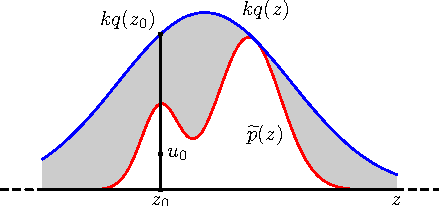
\includegraphics{Figure_4.pdf}
    \end{figure}
\end{frame}

\begin{frame}
    \frametitle{Rejection sampling}
    Let's verify the correctness of the rejection sampling method. Suppose that random variable $Z$ is distributed according to $q(z)$, and random variable $U$ is uniformly distributed over $[0,kq(Z)]$. We want to calculate the probability density function of the random variable $Z|0\le{}U\le\tilde{p}(Z)$:
    \begin{align*}
        P(Z\in{}E|0\le{}U\le\tilde{p}(Z))&=\frac{P(Z\in{}E,0\le{}U\le\tilde{p}(Z))}{P(0\le{}U\le\tilde{p}(Z))} \\
        &=\frac{\int_{E}q(z)\frac{\tilde{p}(z)}{kq(z)}\mathrm{d}z}{\int_{\mathbb{R}}q(z)\frac{\tilde{p}(z)}{kq(z)}\mathrm{d}z} \\
        &=\int_{E}p(z)\mathrm{d}z
    \end{align*}
    We see that the random variable $Z|0\le{}U\le\tilde{p}(Z)$ is indeed distributed according to $p(z)$.
\end{frame}

\begin{frame}
    \frametitle{Rejection sampling}
    Let's calculate the probability that a sample will be accepted:
    \begin{equation*}
        P_{\textrm{accept}}=\int_{\mathbb{R}}q(z)\frac{\tilde{p}(z)}{kq(z)}\mathrm{d}z=\frac{Z_{p}}{k}
    \end{equation*}
    We see that the constant $k$ should be as small as possible subject to the limitation that $kq(z)$ must be nowhere less than $\tilde{p}(z)$.
\end{frame}

\begin{frame}
    \frametitle{Adaptive rejection sampling}
    \begin{itemize}
        \item In many instances, it can be difficult to determine a suitable analytic form for the envelope distribution $q(z)$.
        \item An alternative approach is to construct the envelope function on the fly based on measured values of the distribution $p(z)$.
        \item Constructing an envelope function is particularly straightforward when $p(z)$ is log concave.
    \end{itemize}
\end{frame}

\begin{frame}
    \frametitle{Adaptive rejection sampling}
    \begin{itemize}
        \item Evaluate the function $\log{}p(z)$ and its gradient at some initial set of grid points.
        \item The intersections of the resulting tangent lines are used to construct the envelope function.
        \item Draw a sample value from the envelope distribution. This is straightforward because the envelope function comprises a piecewise exponential distribution.
        \item If the sample is accepted, then it will be a draw from the desired distribution.
        \item If the sample is rejected, then it is incorporated into the set of grid points, a new tangent line is computed, and the envelope function is thereby refined.
    \end{itemize}
\end{frame}

\begin{frame}
    \frametitle{Adaptive rejection sampling}
    \begin{figure}
        \caption{Illustration of the construction of an envelope function for adaptive rejection sampling}
        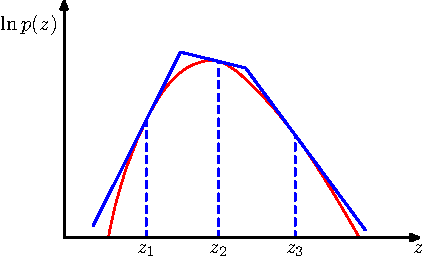
\includegraphics{Figure_6.pdf}
    \end{figure}
\end{frame}

\begin{frame}
    \frametitle{Importance sampling}
    The technique of importance sampling provides a framework for approximating expectations directly but does not itself provide a mechanism for drawing samples from a distribution $p(z)$.
    \bigbreak
    Suppose we wish to calculate the expectation of a function $f(z)$ with respect to a distribution $p(z)$:
    \begin{itemize}
        \item The distribution $p(z)$ can be evaluated only up to a normalization constant, so that $p(z)=\frac{\tilde{p}(z)}{Z_{p}}$, where $Z_{p}$ is unknown.
        \item Because it is difficult to draw samples directly from $p(z)$, we rely on a proposal distribution $q(z)$ from which it is easy to draw samples.
        \item The distribution $q(z)$ also has an unknown normalization constant $Z_{q}$, so that $q(z)=\frac{\tilde{q}(z)}{Z_{q}}$.
    \end{itemize}
\end{frame}

\begin{frame}
    \frametitle{Importance sampling}
    Let's calculate the expectation of $f(z)$ with respect to $p(z)$:
    \begin{align*}
        E(f)&=\int{}f(z)p(z)\mathrm{d}z=\int{}f(z)\frac{p(z)}{q(z)}q(z)\mathrm{d}z \\
        &\approx\frac{1}{L}\sum_{l=1}^{L}f(z^{(l)})\frac{p(z^{(l)})}{q(z^{(l)})}=\frac{Z_{q}}{Z_{p}}\frac{1}{L}\sum_{l=1}^{L}f(z^{(l)})\frac{\tilde{p}(z^{(l)})}{\tilde{q}(z^{(l)})} \\
        \frac{Z_{p}}{Z_{q}}&=\frac{1}{Z_{q}}\int\tilde{p}(z)\mathrm{d}z=\frac{1}{Z_{q}}\int\frac{\tilde{p}(z)}{q(z)}q(z)\mathrm{d}z \\
        &\approx\frac{1}{Z_{q}}\frac{1}{L}\sum_{l=1}^{L}\frac{\tilde{p}(z^{(l)})}{q(z^{(l)})}=\frac{1}{L}\sum_{l=1}^{L}\frac{\tilde{p}(z^{(l)})}{\tilde{q}(z^{(l)})}
    \end{align*}
    where the samples $\{z^{(l)}\}$ are drawn from $q(z)$.
\end{frame}

\begin{frame}
    \frametitle{Importance sampling}
    Let:
    \begin{align*}
        \tilde{r}_{l}&=\frac{\tilde{p}(z^{(l)})}{\tilde{q}(z^{(l)})} \\
        w_{l}&=\frac{\tilde{r}_{l}}{\sum_{l'}\tilde{r}_{l'}}
    \end{align*}
    we see that:
    \begin{equation*}
        E(f)\approx\frac{\sum_{l=1}^{L}f(z^{(l)})\tilde{r}_{l}}{\sum_{l=1}^{L}\tilde{r}_{l}}=\sum_{l=1}^{L}w_{l}f(z^{(l)})
    \end{equation*}
\end{frame}

\begin{frame}
    \frametitle{Sampling-importance-resampling}
    \begin{itemize}
        \item Draw $L$ samples $z^{(1)},\hdots,z^{(L)}$ from $q(z)$.
        \item Construct weights $w_{1},\hdots,w_{L}$ using $w_{l}=\frac{\tilde{r}_{l}}{\sum_{l'}\tilde{r}_{l'}}=\frac{\tilde{p}(z^{(l)})/q(z^{(l)})}{\sum_{l'}\tilde{p}(z^{(l')})/q(z^{(l')})}$.
        \item Draw $L$ samples from the discrete distribution $(z^{(1)},\hdots,z^{(L)})$ with probabilities given by the weights $(w_{1},\hdots,w_{L})$.
    \end{itemize}
\end{frame}

\begin{frame}
    \frametitle{Sampling-importance-resampling}
    Let's verify the correctness of the sampling-importance-resampling method.
    \begin{equation*}
        P(z\le{}a)=\sum_{l=1}^{L}I(z^{(l)}\le{}a)w_{l}=\frac{\sum_{l=1}^{L}I(z^{(l)}\le{}a)\frac{\tilde{p}(z^{(l)})}{q(z^{(l)})}}{\sum_{l=1}^{L}\frac{\tilde{p}(z^{(l)})}{q(z^{(l)})}}
    \end{equation*}
    where $I$ is the indicator function. Taking the limit $L\to\infty$:
    \begin{align*}
        P(z\le{}a)&=\frac{\int{}I(z\le{}a)\frac{\tilde{p}(z)}{q(z)}q(z)\mathrm{d}z}{\int\frac{\tilde{p}(z)}{q(z)}q(z)\mathrm{d}z}=\frac{\int_{-\infty}^{a}\tilde{p}(z)\mathrm{d}z}{\int_{-\infty}^{\infty}\tilde{p}(z)\mathrm{d}z}=\int_{-\infty}^{a}p(z)\mathrm{d}z
    \end{align*}
\end{frame}

\end{document}